\documentclass[11pt,]{article}
\usepackage{lmodern}
\usepackage{amssymb,amsmath}
\usepackage{ifxetex,ifluatex}
\usepackage{fixltx2e} % provides \textsubscript
\ifnum 0\ifxetex 1\fi\ifluatex 1\fi=0 % if pdftex
  \usepackage[T1]{fontenc}
  \usepackage[utf8]{inputenc}
\else % if luatex or xelatex
  \ifxetex
    \usepackage{mathspec}
  \else
    \usepackage{fontspec}
  \fi
  \defaultfontfeatures{Ligatures=TeX,Scale=MatchLowercase}
\fi
% use upquote if available, for straight quotes in verbatim environments
\IfFileExists{upquote.sty}{\usepackage{upquote}}{}
% use microtype if available
\IfFileExists{microtype.sty}{%
\usepackage{microtype}
\UseMicrotypeSet[protrusion]{basicmath} % disable protrusion for tt fonts
}{}
\usepackage[margin=.75in]{geometry}
\usepackage{hyperref}
\hypersetup{unicode=true,
            pdftitle={Problem Set \#3},
            pdfauthor={Anaya Hall \& Christian Miller},
            pdfborder={0 0 0},
            breaklinks=true}
\urlstyle{same}  % don't use monospace font for urls
\usepackage{color}
\usepackage{fancyvrb}
\newcommand{\VerbBar}{|}
\newcommand{\VERB}{\Verb[commandchars=\\\{\}]}
\DefineVerbatimEnvironment{Highlighting}{Verbatim}{commandchars=\\\{\}}
% Add ',fontsize=\small' for more characters per line
\usepackage{framed}
\definecolor{shadecolor}{RGB}{248,248,248}
\newenvironment{Shaded}{\begin{snugshade}}{\end{snugshade}}
\newcommand{\KeywordTok}[1]{\textcolor[rgb]{0.13,0.29,0.53}{\textbf{#1}}}
\newcommand{\DataTypeTok}[1]{\textcolor[rgb]{0.13,0.29,0.53}{#1}}
\newcommand{\DecValTok}[1]{\textcolor[rgb]{0.00,0.00,0.81}{#1}}
\newcommand{\BaseNTok}[1]{\textcolor[rgb]{0.00,0.00,0.81}{#1}}
\newcommand{\FloatTok}[1]{\textcolor[rgb]{0.00,0.00,0.81}{#1}}
\newcommand{\ConstantTok}[1]{\textcolor[rgb]{0.00,0.00,0.00}{#1}}
\newcommand{\CharTok}[1]{\textcolor[rgb]{0.31,0.60,0.02}{#1}}
\newcommand{\SpecialCharTok}[1]{\textcolor[rgb]{0.00,0.00,0.00}{#1}}
\newcommand{\StringTok}[1]{\textcolor[rgb]{0.31,0.60,0.02}{#1}}
\newcommand{\VerbatimStringTok}[1]{\textcolor[rgb]{0.31,0.60,0.02}{#1}}
\newcommand{\SpecialStringTok}[1]{\textcolor[rgb]{0.31,0.60,0.02}{#1}}
\newcommand{\ImportTok}[1]{#1}
\newcommand{\CommentTok}[1]{\textcolor[rgb]{0.56,0.35,0.01}{\textit{#1}}}
\newcommand{\DocumentationTok}[1]{\textcolor[rgb]{0.56,0.35,0.01}{\textbf{\textit{#1}}}}
\newcommand{\AnnotationTok}[1]{\textcolor[rgb]{0.56,0.35,0.01}{\textbf{\textit{#1}}}}
\newcommand{\CommentVarTok}[1]{\textcolor[rgb]{0.56,0.35,0.01}{\textbf{\textit{#1}}}}
\newcommand{\OtherTok}[1]{\textcolor[rgb]{0.56,0.35,0.01}{#1}}
\newcommand{\FunctionTok}[1]{\textcolor[rgb]{0.00,0.00,0.00}{#1}}
\newcommand{\VariableTok}[1]{\textcolor[rgb]{0.00,0.00,0.00}{#1}}
\newcommand{\ControlFlowTok}[1]{\textcolor[rgb]{0.13,0.29,0.53}{\textbf{#1}}}
\newcommand{\OperatorTok}[1]{\textcolor[rgb]{0.81,0.36,0.00}{\textbf{#1}}}
\newcommand{\BuiltInTok}[1]{#1}
\newcommand{\ExtensionTok}[1]{#1}
\newcommand{\PreprocessorTok}[1]{\textcolor[rgb]{0.56,0.35,0.01}{\textit{#1}}}
\newcommand{\AttributeTok}[1]{\textcolor[rgb]{0.77,0.63,0.00}{#1}}
\newcommand{\RegionMarkerTok}[1]{#1}
\newcommand{\InformationTok}[1]{\textcolor[rgb]{0.56,0.35,0.01}{\textbf{\textit{#1}}}}
\newcommand{\WarningTok}[1]{\textcolor[rgb]{0.56,0.35,0.01}{\textbf{\textit{#1}}}}
\newcommand{\AlertTok}[1]{\textcolor[rgb]{0.94,0.16,0.16}{#1}}
\newcommand{\ErrorTok}[1]{\textcolor[rgb]{0.64,0.00,0.00}{\textbf{#1}}}
\newcommand{\NormalTok}[1]{#1}
\usepackage{longtable,booktabs}
\usepackage{graphicx,grffile}
\makeatletter
\def\maxwidth{\ifdim\Gin@nat@width>\linewidth\linewidth\else\Gin@nat@width\fi}
\def\maxheight{\ifdim\Gin@nat@height>\textheight\textheight\else\Gin@nat@height\fi}
\makeatother
% Scale images if necessary, so that they will not overflow the page
% margins by default, and it is still possible to overwrite the defaults
% using explicit options in \includegraphics[width, height, ...]{}
\setkeys{Gin}{width=\maxwidth,height=\maxheight,keepaspectratio}
\IfFileExists{parskip.sty}{%
\usepackage{parskip}
}{% else
\setlength{\parindent}{0pt}
\setlength{\parskip}{6pt plus 2pt minus 1pt}
}
\setlength{\emergencystretch}{3em}  % prevent overfull lines
\providecommand{\tightlist}{%
  \setlength{\itemsep}{0pt}\setlength{\parskip}{0pt}}
\setcounter{secnumdepth}{0}
% Redefines (sub)paragraphs to behave more like sections
\ifx\paragraph\undefined\else
\let\oldparagraph\paragraph
\renewcommand{\paragraph}[1]{\oldparagraph{#1}\mbox{}}
\fi
\ifx\subparagraph\undefined\else
\let\oldsubparagraph\subparagraph
\renewcommand{\subparagraph}[1]{\oldsubparagraph{#1}\mbox{}}
\fi

%%% Use protect on footnotes to avoid problems with footnotes in titles
\let\rmarkdownfootnote\footnote%
\def\footnote{\protect\rmarkdownfootnote}

%%% Change title format to be more compact
\usepackage{titling}

% Create subtitle command for use in maketitle
\newcommand{\subtitle}[1]{
  \posttitle{
    \begin{center}\large#1\end{center}
    }
}

\setlength{\droptitle}{-2em}
  \title{Problem Set \#3}
  \pretitle{\vspace{\droptitle}\centering\huge}
  \posttitle{\par}
  \author{Anaya Hall \& Christian Miller}
  \preauthor{\centering\large\emph}
  \postauthor{\par}
  \predate{\centering\large\emph}
  \postdate{\par}
  \date{Due approximately April 6th}

\usepackage{booktabs}
\usepackage{longtable}
\usepackage{array}
\usepackage{multirow}
\usepackage[table]{xcolor}
\usepackage{wrapfig}
\usepackage{float}
\usepackage{colortbl}
\usepackage{pdflscape}
\usepackage{tabu}
\usepackage{threeparttable}
\usepackage[normalem]{ulem}

\begin{document}
\maketitle

\section{Wage Regressions - Blackburn and Neumark (QJE
1992)}\label{wage-regressions---blackburn-and-neumark-qje-1992}

The goal of this problem set is to explore some \textbf{tests for
heteroskedasticity} and explore \textbf{the fixes} discussed in class.

\subsection{Question 1:}\label{question-1}

\textbf{Read the data into R. Plot the series and make sure your data
are read in correctly.}

\begin{Shaded}
\begin{Highlighting}[]
\CommentTok{# Read in CSV as data.frame}
\NormalTok{wage_df <-}\StringTok{ }\NormalTok{readr}\OperatorTok{::}\KeywordTok{read_csv}\NormalTok{(}\StringTok{"nls80.csv"}\NormalTok{)}

\CommentTok{# Select only the variables in our model}
\NormalTok{wage_df }\OperatorTok\StringTok{ }\KeywordTok{select}\NormalTok{(wage, exper, tenure, married, south, urban, black, educ)}
\end{Highlighting}
\end{Shaded}

\begin{Shaded}
\begin{Highlighting}[]
\CommentTok{# Plot the variables in our model}
\KeywordTok{ggplot}\NormalTok{(}\DataTypeTok{data =} \KeywordTok{gather}\NormalTok{(wage_df), }\KeywordTok{aes}\NormalTok{(}\DataTypeTok{x =}\NormalTok{ value)) }\OperatorTok{+}
\KeywordTok{geom_histogram}\NormalTok{() }\OperatorTok{+}
\KeywordTok{facet_wrap}\NormalTok{(}\OperatorTok{~}\StringTok{ }\NormalTok{key, }\DataTypeTok{scales =} \StringTok{"free"}\NormalTok{) }\OperatorTok{+}
\KeywordTok{ggtitle}\NormalTok{(}\StringTok{"Histograms of Wage Data variables"}\NormalTok{) }\OperatorTok{+}
\KeywordTok{ylab}\NormalTok{(}\StringTok{"Count"}\NormalTok{) }\OperatorTok{+}
\KeywordTok{xlab}\NormalTok{(}\StringTok{"Value"}\NormalTok{) }\OperatorTok{+}\StringTok{ }\KeywordTok{theme_minimal}\NormalTok{()}
\end{Highlighting}
\end{Shaded}

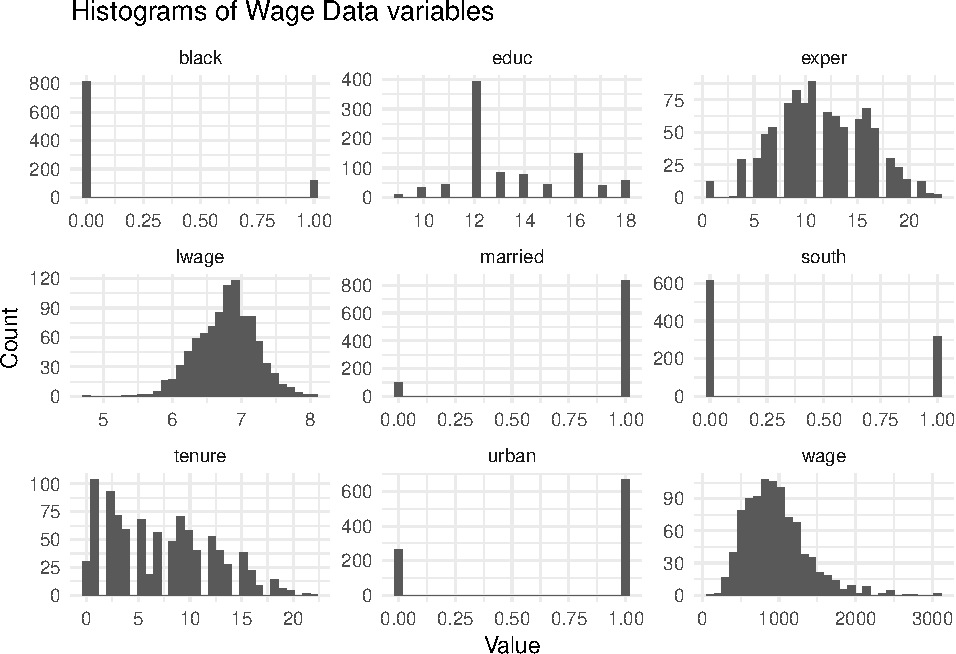
\includegraphics{ps3_code_files/figure-latex/plot_series-1.pdf}

So far, everthing looks good.

\subsection{Question 2: Exploring
Heteroskedasticity}\label{question-2-exploring-heteroskedasticity}

Model (1) :

\(log(wage) = \beta_0 + exper \cdot \beta_1 + tenure \cdot \beta_2 + married \cdot \beta_3 + south \cdot \beta_4 + urban \cdot \beta_5 + black \cdot \beta_6 + educ \cdot \beta_7 + \epsilon\)

\subsubsection{(a) Estimate model (1) via
OLS}\label{a-estimate-model-1-via-ols}

First, load our OLS function created in Problem Sets 1 \& 2.

\begin{Shaded}
\begin{Highlighting}[]
\CommentTok{# Function to convert tibble, data.frame, or tbl_df to matrix}
\NormalTok{to_matrix <-}\StringTok{ }\ControlFlowTok{function}\NormalTok{(the_df, vars) \{}
  \CommentTok{# Create a matrix from variables in var}
\NormalTok{  new_mat <-}\StringTok{ }\NormalTok{the_df }\OperatorTok
\StringTok{    }\CommentTok{#Select the columns given in 'vars'}
\StringTok{    }\KeywordTok{select_}\NormalTok{(}\DataTypeTok{.dots =}\NormalTok{ vars) }\OperatorTok
\StringTok{    }\CommentTok{# Convert to matrix}
\StringTok{    }\KeywordTok{as.matrix}\NormalTok{()}
  \CommentTok{# Return 'new_mat'}
  \KeywordTok{return}\NormalTok{(new_mat)}
\NormalTok{\}}

\NormalTok{ols <-}\StringTok{ }\ControlFlowTok{function}\NormalTok{(data, y_data, X_data, }\DataTypeTok{intercept =}\NormalTok{ T, }\DataTypeTok{H0 =} \DecValTok{0}\NormalTok{, }\DataTypeTok{two_tail =}\NormalTok{ T, }\DataTypeTok{alpha =} \FloatTok{0.05}\NormalTok{) \{}
  \CommentTok{# Function setup ----}
    \CommentTok{# Require the 'dplyr' package}
    \KeywordTok{require}\NormalTok{(dplyr)}
  
  \CommentTok{# Create dependent and independent variable matrices ----}
    \CommentTok{# y matrix}
\NormalTok{    y <-}\StringTok{ }\KeywordTok{to_matrix}\NormalTok{ (}\DataTypeTok{the_df =}\NormalTok{ data, }\DataTypeTok{vars =}\NormalTok{ y_data)}
    \CommentTok{# X matrix}
\NormalTok{    X <-}\StringTok{ }\KeywordTok{to_matrix}\NormalTok{ (}\DataTypeTok{the_df =}\NormalTok{ data, }\DataTypeTok{vars =}\NormalTok{ X_data)}
      \CommentTok{# If 'intercept' is TRUE, then add a column of ones}
      \ControlFlowTok{if}\NormalTok{ (intercept }\OperatorTok{==}\StringTok{ }\NormalTok{T) \{}
\NormalTok{      X <-}\StringTok{ }\KeywordTok{cbind}\NormalTok{(}\DecValTok{1}\NormalTok{,X)}
      \KeywordTok{colnames}\NormalTok{(X) <-}\StringTok{ }\KeywordTok{c}\NormalTok{(}\StringTok{"intercept"}\NormalTok{, X_data)}
\NormalTok{      \}}
 
  \CommentTok{# Calculate b, y_hat, and residuals ----}
\NormalTok{    b <-}\StringTok{ }\KeywordTok{solve}\NormalTok{(}\KeywordTok{t}\NormalTok{(X) }\OperatorTok\StringTok{ }\NormalTok{X) }\OperatorTok\StringTok{ }\KeywordTok{t}\NormalTok{(X) }\OperatorTok\StringTok{ }\NormalTok{y}
\NormalTok{    y_hat <-}\StringTok{ }\NormalTok{X }\OperatorTok\StringTok{ }\NormalTok{b}
\NormalTok{    e <-}\StringTok{ }\NormalTok{y }\OperatorTok{-}\StringTok{ }\NormalTok{y_hat}
    
  \CommentTok{# Useful -----}
\NormalTok{    n <-}\StringTok{ }\KeywordTok{nrow}\NormalTok{(X) }\CommentTok{# number of observations}
\NormalTok{    k <-}\StringTok{ }\KeywordTok{ncol}\NormalTok{(X) }\CommentTok{# number of independent variables}
\NormalTok{    dof <-}\StringTok{ }\NormalTok{n }\OperatorTok{-}\StringTok{ }\NormalTok{k }\CommentTok{# degrees of freedom}
\NormalTok{    i <-}\StringTok{ }\KeywordTok{rep}\NormalTok{(}\DecValTok{1}\NormalTok{,n) }\CommentTok{# column of ones for demeaning matrix}
\NormalTok{    A <-}\StringTok{ }\KeywordTok{diag}\NormalTok{(i) }\OperatorTok{-}\StringTok{ }\NormalTok{(}\DecValTok{1} \OperatorTok{/}\StringTok{ }\NormalTok{n) }\OperatorTok{*}\StringTok{ }\NormalTok{i }\OperatorTok\StringTok{ }\KeywordTok{t}\NormalTok{(i) }\CommentTok{# demeaning matrix}
\NormalTok{    y_star <-}\StringTok{ }\NormalTok{A }\OperatorTok\StringTok{ }\NormalTok{y }\CommentTok{# for SST}
\NormalTok{    X_star <-}\StringTok{ }\NormalTok{A }\OperatorTok\StringTok{ }\NormalTok{X }\CommentTok{# for SSM}
\NormalTok{    SST <-}\StringTok{ }\KeywordTok{drop}\NormalTok{(}\KeywordTok{t}\NormalTok{(y_star) }\OperatorTok\StringTok{ }\NormalTok{y_star)}
\NormalTok{    SSM <-}\StringTok{ }\KeywordTok{drop}\NormalTok{(}\KeywordTok{t}\NormalTok{(b) }\OperatorTok\StringTok{ }\KeywordTok{t}\NormalTok{(X_star) }\OperatorTok\StringTok{ }\NormalTok{X_star }\OperatorTok\StringTok{ }\NormalTok{b)}
\NormalTok{    SSR <-}\StringTok{ }\KeywordTok{drop}\NormalTok{(}\KeywordTok{t}\NormalTok{(e) }\OperatorTok\StringTok{ }\NormalTok{e)}
  
  \CommentTok{# Measures of fit and estimated variance ----}
\NormalTok{    R2uc <-}\StringTok{ }\KeywordTok{drop}\NormalTok{((}\KeywordTok{t}\NormalTok{(y_hat) }\OperatorTok\StringTok{ }\NormalTok{y_hat)}\OperatorTok{/}\NormalTok{(}\KeywordTok{t}\NormalTok{(y) }\OperatorTok\StringTok{ }\NormalTok{y)) }\CommentTok{# Uncentered R^2}
\NormalTok{    R2 <-}\StringTok{ }\DecValTok{1} \OperatorTok{-}\StringTok{ }\NormalTok{SSR}\OperatorTok{/}\NormalTok{SST }\CommentTok{# Uncentered R^2}
\NormalTok{    R2adj <-}\StringTok{ }\DecValTok{1} \OperatorTok{-}\StringTok{ }\NormalTok{(n}\OperatorTok{-}\DecValTok{1}\NormalTok{)}\OperatorTok{/}\NormalTok{dof }\OperatorTok{*}\StringTok{ }\NormalTok{(}\DecValTok{1} \OperatorTok{-}\StringTok{ }\NormalTok{R2) }\CommentTok{# Adjusted R^2}
\NormalTok{    AIC <-}\StringTok{ }\KeywordTok{log}\NormalTok{(SSR}\OperatorTok{/}\NormalTok{n) }\OperatorTok{+}\StringTok{ }\DecValTok{2}\OperatorTok{*}\NormalTok{k}\OperatorTok{/}\NormalTok{n }\CommentTok{# AIC}
\NormalTok{    SIC <-}\StringTok{ }\KeywordTok{log}\NormalTok{(SSR}\OperatorTok{/}\NormalTok{n) }\OperatorTok{+}\StringTok{ }\NormalTok{k}\OperatorTok{/}\NormalTok{n}\OperatorTok{*}\KeywordTok{log}\NormalTok{(n) }\CommentTok{# SIC}
\NormalTok{    s2 <-}\StringTok{ }\NormalTok{SSR}\OperatorTok{/}\NormalTok{dof }\CommentTok{# s^2}
  
  \CommentTok{# Measures of fit table ----}
\NormalTok{    mof_table_df <-}\StringTok{ }\KeywordTok{data.frame}\NormalTok{(R2uc, R2, R2adj, SIC, AIC, SSR, s2)}
\NormalTok{    mof_table_col_names <-}\StringTok{ }\KeywordTok{c}\NormalTok{(}\StringTok{"$R^2_}\CharTok{\textbackslash{}\textbackslash{}}\StringTok{text\{uc\}$"}\NormalTok{, }\StringTok{"$R^2$"}\NormalTok{,}
                             \StringTok{"$R^2_}\CharTok{\textbackslash{}\textbackslash{}}\StringTok{text\{adj\}$"}\NormalTok{,}
                             \StringTok{"SIC"}\NormalTok{, }\StringTok{"AIC"}\NormalTok{, }\StringTok{"SSR"}\NormalTok{, }\StringTok{"$s^2$"}\NormalTok{)}
\NormalTok{    mof_table <-}\StringTok{  }\NormalTok{mof_table_df }\OperatorTok\StringTok{ }\NormalTok{knitr}\OperatorTok{::}\KeywordTok{kable}\NormalTok{(}
      \DataTypeTok{row.names =}\NormalTok{ F,}
      \DataTypeTok{col.names =}\NormalTok{ mof_table_col_names,}
      \DataTypeTok{format.args =} \KeywordTok{list}\NormalTok{(}\DataTypeTok{scientific =}\NormalTok{ F, }\DataTypeTok{digits =} \DecValTok{4}\NormalTok{),}
      \DataTypeTok{booktabs =}\NormalTok{ T,}
      \DataTypeTok{escape =}\NormalTok{ F}
\NormalTok{    )}
  
  \CommentTok{# t-test----}
    \CommentTok{# Standard error}
\NormalTok{    se <-}\StringTok{ }\KeywordTok{as.vector}\NormalTok{(}\KeywordTok{sqrt}\NormalTok{(s2 }\OperatorTok{*}\StringTok{ }\KeywordTok{diag}\NormalTok{(}\KeywordTok{solve}\NormalTok{(}\KeywordTok{t}\NormalTok{(X) }\OperatorTok\StringTok{ }\NormalTok{X))))}
    \CommentTok{# Vector of _t_ statistics}
\NormalTok{    t_stats <-}\StringTok{ }\NormalTok{(b }\OperatorTok{-}\StringTok{ }\NormalTok{H0) }\OperatorTok{/}\StringTok{ }\NormalTok{se}
    \CommentTok{# Calculate the p-values}
    \ControlFlowTok{if}\NormalTok{ (two_tail }\OperatorTok{==}\StringTok{ }\NormalTok{T) \{}
\NormalTok{    p_values <-}\StringTok{ }\KeywordTok{pt}\NormalTok{(}\DataTypeTok{q =} \KeywordTok{abs}\NormalTok{(t_stats), }\DataTypeTok{df =}\NormalTok{ dof, }\DataTypeTok{lower.tail =}\NormalTok{ F) }\OperatorTok{*}\StringTok{ }\DecValTok{2}
\NormalTok{    \} }\ControlFlowTok{else}\NormalTok{ \{}
\NormalTok{      p_values <-}\StringTok{ }\KeywordTok{pt}\NormalTok{(}\DataTypeTok{q =} \KeywordTok{abs}\NormalTok{(t_stats), }\DataTypeTok{df =}\NormalTok{ dof, }\DataTypeTok{lower.tail =}\NormalTok{ F)}
\NormalTok{    \}}
    \CommentTok{# Do we (fail to) reject?}
\NormalTok{    reject <-}\StringTok{ }\KeywordTok{ifelse}\NormalTok{(p_values }\OperatorTok{<}\StringTok{ }\NormalTok{alpha, reject <-}\StringTok{ "Reject"}\NormalTok{, reject <-}\StringTok{ "Fail to Reject"}\NormalTok{)}
    
    \CommentTok{# Nice table (data.frame) of results}
\NormalTok{    ttest_df <-}\StringTok{ }\KeywordTok{data.frame}\NormalTok{(}
      \CommentTok{# The rows have the coef. names}
      \DataTypeTok{effect =} \KeywordTok{rownames}\NormalTok{(b),}
      \CommentTok{# Estimated coefficients}
      \DataTypeTok{coef =} \KeywordTok{as.vector}\NormalTok{(b) }\OperatorTok\StringTok{ }\KeywordTok{round}\NormalTok{(}\DecValTok{3}\NormalTok{),}
      \CommentTok{# Standard errors}
      \DataTypeTok{std_error =} \KeywordTok{as.vector}\NormalTok{(se) }\OperatorTok\StringTok{ }\KeywordTok{round}\NormalTok{(}\DecValTok{3}\NormalTok{),}
      \CommentTok{# t statistics}
      \DataTypeTok{t_stat =} \KeywordTok{as.vector}\NormalTok{(t_stats) }\OperatorTok\StringTok{ }\KeywordTok{round}\NormalTok{(}\DecValTok{3}\NormalTok{),}
      \CommentTok{# p-values}
      \DataTypeTok{p_value =} \KeywordTok{as.vector}\NormalTok{(p_values) }\OperatorTok\StringTok{ }\KeywordTok{round}\NormalTok{(}\DecValTok{4}\NormalTok{),}
      \CommentTok{# reject null?}
      \DataTypeTok{significance =} \KeywordTok{as.character}\NormalTok{(reject)}
\NormalTok{      )}
  
\NormalTok{    ttest_table <-}\StringTok{  }\NormalTok{ttest_df }\OperatorTok\StringTok{ }\NormalTok{knitr}\OperatorTok{::}\KeywordTok{kable}\NormalTok{(}
      \DataTypeTok{booktabs =}\NormalTok{ T,}
      \DataTypeTok{format.args =} \KeywordTok{list}\NormalTok{(}\DataTypeTok{scientific =}\NormalTok{ F),}
      \DataTypeTok{escape =}\NormalTok{ F,}
      \DataTypeTok{caption =} \StringTok{"OLS Results"}
\NormalTok{    )}

  \CommentTok{# Data frame for exporting for y, y_hat, X, and e vectors ----}
\NormalTok{    export_df <-}\StringTok{ }\KeywordTok{data.frame}\NormalTok{(y, y_hat, e, X) }\OperatorTok\StringTok{ }\KeywordTok{tbl_df}\NormalTok{()}
    \KeywordTok{colnames}\NormalTok{(export_df) <-}\StringTok{ }\KeywordTok{c}\NormalTok{(}\StringTok{"y"}\NormalTok{,}\StringTok{"y_hat"}\NormalTok{,}\StringTok{"e"}\NormalTok{,}\KeywordTok{colnames}\NormalTok{(X))}
  
  \CommentTok{# Return ----}
    \KeywordTok{return}\NormalTok{(}\KeywordTok{list}\NormalTok{(}\DataTypeTok{n=}\NormalTok{n, }\DataTypeTok{dof=}\NormalTok{dof, }\DataTypeTok{b=}\NormalTok{b, }\DataTypeTok{vars=}\NormalTok{export_df, }\DataTypeTok{resid=}\NormalTok{e, }\DataTypeTok{R2uc=}\NormalTok{R2uc,}\DataTypeTok{R2=}\NormalTok{R2,}
                \DataTypeTok{R2adj=}\NormalTok{R2adj, }\DataTypeTok{AIC=}\NormalTok{AIC, }\DataTypeTok{SIC=}\NormalTok{SIC, }\DataTypeTok{s2=}\NormalTok{s2, }\DataTypeTok{SST=}\NormalTok{SST, }\DataTypeTok{SSR=}\NormalTok{SSR,}
                \DataTypeTok{mof_table=}\NormalTok{mof_table, }\DataTypeTok{ttest=}\NormalTok{ttest_table))}
\NormalTok{\}}
\end{Highlighting}
\end{Shaded}

\newpage

\begin{Shaded}
\begin{Highlighting}[]
\NormalTok{wage_df }\OperatorTok\StringTok{ }\KeywordTok{mutate}\NormalTok{(}
  \DataTypeTok{log_wage =} \KeywordTok{log}\NormalTok{(wage))}

\NormalTok{model_}\DecValTok{1}\NormalTok{ <-}\StringTok{ }\KeywordTok{ols}\NormalTok{(wage_df, }\DataTypeTok{y_data =} \StringTok{"log_wage"}\NormalTok{, }
               \DataTypeTok{X_data =} \KeywordTok{c}\NormalTok{(}\StringTok{"exper"}\NormalTok{, }\StringTok{"tenure"}\NormalTok{, }\StringTok{"married"}\NormalTok{, }\StringTok{"south"}\NormalTok{, }\StringTok{"urban"}\NormalTok{, }\StringTok{"black"}\NormalTok{, }\StringTok{"educ"}\NormalTok{))}

\NormalTok{model_}\DecValTok{1}\OperatorTok{$}\NormalTok{ttest}
\end{Highlighting}
\end{Shaded}

\begin{longtable}[]{@{}lrrrrl@{}}
\caption{OLS Results}\tabularnewline
\toprule
effect & coef & std\_error & t\_stat & p\_value &
significance\tabularnewline
\midrule
\endfirsthead
\toprule
effect & coef & std\_error & t\_stat & p\_value &
significance\tabularnewline
\midrule
\endhead
intercept & 5.395 & 0.113 & 47.653 & 0.0000 & Reject\tabularnewline
exper & 0.014 & 0.003 & 4.409 & 0.0000 & Reject\tabularnewline
tenure & 0.012 & 0.002 & 4.789 & 0.0000 & Reject\tabularnewline
married & 0.199 & 0.039 & 5.107 & 0.0000 & Reject\tabularnewline
south & -0.091 & 0.026 & -3.463 & 0.0006 & Reject\tabularnewline
urban & 0.184 & 0.027 & 6.822 & 0.0000 & Reject\tabularnewline
black & -0.188 & 0.038 & -5.000 & 0.0000 & Reject\tabularnewline
educ & 0.065 & 0.006 & 10.468 & 0.0000 & Reject\tabularnewline
\bottomrule
\end{longtable}

\subsubsection{(b) Conduct a White test for heteroskedastic
errors.}\label{b-conduct-a-white-test-for-heteroskedastic-errors.}

\textbf{Use levels, interactions and second order terms only. Do we have
a problem?}

\emph{White's Test:} Regress the squared residuals (\(e^2_i\)) on a
constant, all variables in \emph{\(X\)}, squares of all variables in
\emph{\(X\)} and all cross products. \(n \dot R^2\) from this regression
is distributed as a \(\chi^2_{(p-1)}\), where p is the number of
regressors in this equation including the constant. The null in this
test is homoskedastic disturbances.

\begin{Shaded}
\begin{Highlighting}[]
\CommentTok{# Prep for white function}
\NormalTok{resid <-}\StringTok{ }\NormalTok{model_}\DecValTok{1}\OperatorTok{$}\NormalTok{resid}
\NormalTok{cov_mat <-}\StringTok{ }\NormalTok{wage_df }\OperatorTok\StringTok{ }\KeywordTok{select}\NormalTok{(exper, tenure, married, south, urban, black, educ)}

\CommentTok{# Run White Test}
\KeywordTok{white_test}\NormalTok{(resid, cov_mat)}
\end{Highlighting}
\end{Shaded}

\begin{verbatim}
## $PValue
## [1] 0.06784352
## 
## $TestStat
## [1] 44.65285
## 
## $dof
## [1] 32
\end{verbatim}

There is some evidence for heteroskedasticity (probabilty is 0.0678),
though not significant at 5\% significance level.

\subsubsection{(c) Goldfeld - Quandt Test for heteroskedastic
errors}\label{c-goldfeld---quandt-test-for-heteroskedastic-errors}

\emph{Use the tenure variable, leaving out the 235 observations in the
middle. Do we have a problem?}

\emph{Goldfeld-Quant Test:} Intuition: The disturbances for two distinct
groups of observations vary.

Process: Rank observations by x, separate into groups of high and low
variances, then calculate test statistic:

\$ F\_{[}n\_1-k, n\_2-k{]} = \frac {e'_1e_1/n_1 -k}{e'_2e_2/n_2 -k} \$

\begin{Shaded}
\begin{Highlighting}[]
\NormalTok{GQ_test <-}\StringTok{ }\ControlFlowTok{function}\NormalTok{(x1, x2) \{}
  
  
  
\NormalTok{\}}
\end{Highlighting}
\end{Shaded}

\subsubsection{(d) Breusch-Pagan Test for heteroskedastic
errors}\label{d-breusch-pagan-test-for-heteroskedastic-errors}

\emph{Use all of the covariates as a simple linear combination. Do we
have a problem?}

\subsection{Question 3: The Delta
Method}\label{question-3-the-delta-method}

See Ed's notes here:
{[}\url{http://edrub.in/ARE212/section09.html\#route_2:_delta_method}{]}

Model (2) :

\$log(wage) = \beta\_0 + exper \cdot \beta\_1 + tenure \cdot \beta\_2 +
married \cdot \beta\_3 + south \cdot \beta\_4 + urban \cdot \beta\_5 +
black \cdot \beta\_6 + educ \cdot \beta\_7 + \epsilon \$


\end{document}
